\documentclass[border=4pt]{standalone}
% Preámbulo común de las figuras. Cada figura es un documento standalone
% que se compila a SVG con scripts/build_figures.sh
\usepackage[utf8]{inputenc}
\usepackage{amsmath}
\usepackage{tikz}
\usepackage[american, siunitx]{circuitikz}
\usetikzlibrary{arrows.meta,calc,decorations.pathmorphing,patterns}
\tikzset{
  >={Stealth[length=2.2mm]},
  eje/.style={->, thin},
  hilo/.style={thick},
}
% Paleta común: tonos medios legibles sobre fondo claro
\definecolor{azul}{RGB}{31,94,168}
\definecolor{rojo}{RGB}{192,57,43}
\definecolor{verde}{RGB}{39,128,73}
\definecolor{naranja}{RGB}{211,120,30}
\definecolor{morado}{RGB}{125,60,152}

\begin{document}
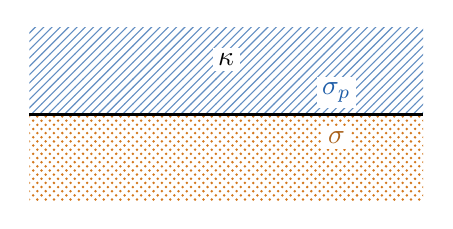
\begin{tikzpicture}[scale=1.0]
  \fill[pattern=north east lines, pattern color=azul!70] (0,0) rectangle (5,1.1);
  \fill[pattern=crosshatch dots, pattern color=naranja] (0,-1.1) rectangle (5,0);
  \draw[very thick] (0,0) -- (5,0);
  \node[fill=white, inner sep=2pt] at (2.5,0.7) {$\kappa$};
  \node[fill=white, inner sep=2pt] at (3.9,0.28) {\color{azul}$\sigma_p$};
  \node[fill=white, inner sep=2pt] at (3.9,-0.3) {\color{naranja!80!black}$\sigma$};
\end{tikzpicture}
\end{document}
